\documentclass[tikz,border=3pt]{standalone}
\usepackage{times}
\usepackage[T1]{fontenc}
\usetikzlibrary{arrows.meta}
\begin{document}
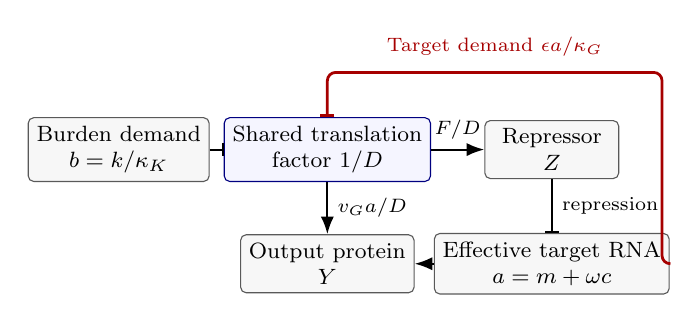
\begin{tikzpicture}[
  x=1cm,y=1cm,>=Latex,
  every node/.style={font=\footnotesize,align=center},
  species/.style={
    draw=black!65,rounded corners=2pt,fill=black!3,
    minimum height=.70cm,inner sep=3pt
  },
  factor/.style={
    species,draw=blue!50!black,fill=blue!4,
    minimum width=1.95cm
  },
  positive/.style={->,line width=.75pt},
  negative/.style={-{Bar[width=5pt]},line width=.75pt},
  demand/.style={
    -{Bar[width=5pt]},line width=1pt,
    draw=red!65!black,rounded corners=3pt
  }
]
  \node[species,minimum width=1.65cm] (b)
    at (-2.65,0) {Burden demand\\$b=k/\kappa_K$};

  \node[factor] (R)
    at (0,0) {Shared translation\\factor $1/D$};

  \node[species,minimum width=1.70cm] (Z)
    at (2.85,0) {Repressor\\$Z$};

  \node[species,minimum width=2.25cm] (a)
    at (2.85,-1.45) {Effective target RNA\\$a=m+\omega c$};

  \node[species,minimum width=1.95cm] (Y)
    at (0,-1.45) {Output protein\\$Y$};

  \draw[negative] (b.east) -- (R.west);

  \draw[positive] (R.east) --
    node[above,font=\scriptsize] {$F/D$}
    (Z.west);

  \draw[positive] (R.south) --
    node[right,font=\scriptsize] {$v_Ga/D$}
    (Y.north);

  \draw[negative] (Z.south) --
    node[right,font=\scriptsize] {repression}
    (a.north);

  \draw[positive] (a.west) -- (Y.east);

  \draw[demand]
    (a.east) -- (4.25,-1.45) -- (4.25,.98)
    -- node[above=2pt,font=\scriptsize,text=red!65!black]
       {Target demand $\epsilon a/\kappa_G$}
    (0,.98) -- (R.north);
\end{tikzpicture}

\end{document}
